\chapter{Casistica, materiali e metodi}

\section{Casistica}

Introduzione alle informazioni della mostrate

\begin{figure}[h]
  \begin{center}
      \includegraphics{grafici/centili/centili} %\\
  \end{center}
  \caption{Standard antropometrici neonatali relativi a peso ed altezza nell'Italia nord-orientale}
\end{figure}

\clearpage

% inizio paziente: non segnare il nome ma le prime due lettere di nome e cognome
\subsection*{Paziente 1} % Ma.Va.

Paziente non dismorfico, senza deficit cognitivo, con familiarità per ritardo costituzionale di crescita. Cresceva per il limite inferiore del bersaglio perentale.
Ha presentato risposta carente a due test provocativi.

\begin{table}[!h]
\begin{tabular}{lrllrl}
\toprule
\multicolumn{6}{l}{\textbf{Dati alla nascita}}\\
Luogo 		& \multicolumn{2}{l}{Torino} 	& Data 					& \multicolumn{2}{l}{28/12/89} 	\\
Sesso 		& \multicolumn{2}{l}{Femmina} 	& Età gestazionale 		& 40 		& sett.\\
Lunghezza 	& 45 		& cm 					& Circonferenza cranica	& 35 		& cm\\
Peso 		& 3350 		& g\\
\midrule
\multicolumn{6}{l}{\textbf{Statura dei genitori}}\\
Padre 		& 165.5 & cm 	& Madre 				& 164.2 & cm \\
MPH 		& ?? 	& cm \\
\midrule
\multicolumn{6}{l}{\textbf{Trattamento con GH}} \\
Età	iniziale	& ?? & 		& Altezza iniziale 				& 135.5 & cm  \\
Peso iniziale	& 25.4 & kg	& Velocità di crescita iniziale & 4.13 & cm/aa\\
Dose media		& ?? & unità & Anni prepuberali trattati		& ??\\
Anni di terapia & ??\\
\midrule
\multicolumn{6}{l}{\textbf{Esito della terapia}} \\
Altezza finale	& ?? & cm 	& SDS guadagnate 			& ??\\
SDS per MPH		& ?? &		& SDS guadagnate per MPH	& ??\\
\bottomrule
\end{tabular}
\end{table}
\clearpage
% fine paziente. il clear page serve a collocare le tabelle prima del paziente successivo.

% inizio paziente
\subsection*{Paziente 2}% Pa. Gi.

Paziente con ritardo di crescita intrauterino (IUGR) da insufficienza placentare.
Presentava dismorfismi (cubito valgo, clinodattilia lieve, palato ogivale, voluminosi padiglioni auricolari) non ascrivibili ad alcuna sindrome genetica. La produzione di GH è risultata carente dopo due test provocativi. Avendo iniziato la pubertà (B2, PH2) ad una statura di 120 cm, è stata effettuata una terapia combinata con GH biosintetico e LHRH analogo. La terapia con LHRH analogo è stata effettuata per un anno e mezzo circa, fino al raggiungimento di una statura pari a 129,6 cm.

\clearpage
% fine paziente. il clear page serve a collocare le tabelle prima del paziente successivo.

% inizio paziente
\subsection*{Paziente 3}% Sc. Fl.

Paziente con glaucoma congenito, lieve clinodattilia e familiarità per bassa statura. Ha presentato insufficiente secrezione di GH  dopo due test provocativi.

\clearpage
% fine paziente. il clear page serve a collocare le tabelle prima del paziente successivo.

% inizio paziente
\subsection*{Paziente 4}% Za. Gi.

Paziente non dismorfico, senza deficit cognitivo. La sua produzione di ormone della crescita è risultata deficitaria dopo due test provocativi.

\clearpage
% fine paziente. il clear page serve a collocare le tabelle prima del paziente successivo.

% inizio paziente
\subsection*{Paziente 5}% Ze. Lu.

Paziente con brachidattilia (come il padre) e con familiarità per bassa statura. Il picco di ormone della crescita è risultato al di sotto del limite inferiore della norma dopo due test provocativi. 

\section{Materiali e metodi}

\subsection{Valutazione auxologica}
Tutti i pazienti sono stati sottoposti a valutazione auxologica prima dell'inizio della terapia, durante e al termine di questa . Infine sono stati valutati a fine crescita. Le misurazioni durante la terapia sono state effettuate a distanza di sei mesi una dall'altra.
%Le variabili auxologiche rilevate comprendono:

\subsubsection*{Statura da eretto}
\`E la distanza verticale dal vertice alla pianta del piede. Il vertice è il punto più alto della testa, quando questa è orientata nella posizione di Francoforte (il margine inferiore dell'orbita e il margine superiore dell'apertura del condotto uditivo sono situati sullo stesso piano orizzontale). La misurazione viene effettuata con lo statimetro di Harpenden; la misura è espressa in centimetri e millimetri.
\begin{figure}[h]
  \begin{center}
	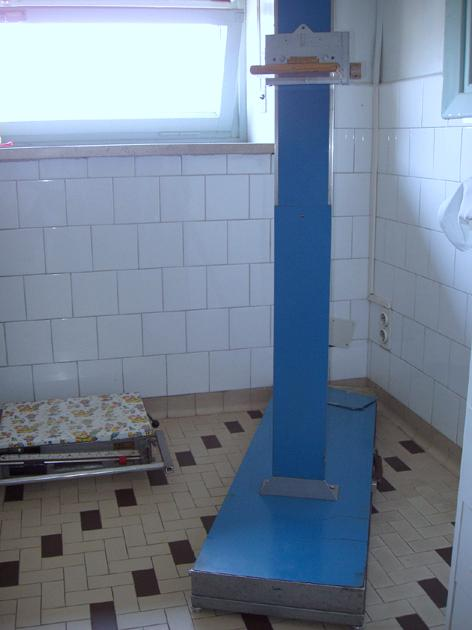
\includegraphics[scale=0.40]{grafici/statimetro.jpg}
  \end{center}
  \caption{Statimetro di Harpenden}
\end{figure}
La tecnica per il rilievo della statura da eretto è la seguente: il soggetto deve stare in piedi, con i talloni vicini fra loro e con i calcagni, le natiche e le spalle appoggiati al piano verticale dello statimetro. I piedi sono leggermente divaricati, in modo da formare un angolo di circa 45 gradi; il soggetto non indossa i propri calzini, ma un paio di sottili calzari in plastica, al fine di ridurre lo spessore. La testa viene orientata nella posizione di Francoforte. Al momento della misurazione il soggetto viene invitato a compiere un'inspirazione profonda, mentre l'osservatore lo tiene in distensione esercitando una trazione verso l'alto con il dito medio di ciascuna mano posto sotto i processi mastoidei. La statura si legge sull'apposito indicatore durante la successiva espirazione, mantenendo la pressione sotto i processi mastoidei%figure con Vannelli.

\subsubsection*{Peso}
Rappresenta l'insieme della massa magra e di quella adiposa. Deve essere rilevato mediante una bilancia tarata che assicuri un approssimazione di kg 0,1. Il soggetto viene pesato con il minimo di indumenti, possibilmente al mattino dopo aver urinato.

\subsubsection*{Velocità di crescita staturale}
Rappresenta l'accrescimento staturale avvenuto in un determinato periodo di tempo. Per calcolarla occorre dividere la differenza fra due misurazioni per l'intervallo di tempo fra queste misurazioni. L'intervallo non deve essere nè troppo breve nè molto lungo: in genere la velocità di crescita staturale si calcola su 6 mesi.

\subsubsection*{Stadi puberali}
Sono un'importante indicatore di maturazione nel periodo puberale\cite{benso2001auxologia}. Nei maschi si rilevano lo stadio dello sviluppo pilifero al pube e dello sviluppo dei genitali; nelle femmine lo sviluppo pilfero al pube e lo sviluppo mammario. Generalmente viene adottata la classificazione di Tanner (1981) in cinque stadi.

\begin{table}[!h]
\begin{tabular}{lp{13.3cm}}
\toprule
\multicolumn{2}{c}{\textbf{Stadi dello sviluppo pilifero al pube (\emph{Pubic Hair})}}\\
PH1 &	preadolescente. Assenza di peli pubici o presenza di lieve peluria lanuginosa.\\
PH2 &	crescita sparsa dei primi peli lunghi, poco pigmentati che appaiono 
		in particolare alla base del pene o lungo le grandi labbra.\\
PH3 &	peli molto più scuri, più ruvidi e più crespi. 
		I peli si diffondono sparsi, sopra il pube.\\
PH4 &	i peli assomigliano al tipo proprio degli adulti ma non vi è diffusione 
		alla superficie mediale delle cosce.\\
PH5 &	configurazione da adulto per quantità e con distribuzione di tipo 
		orizzontale nelle femmine e diffusione lungo la linea
		alba nei maschi; diffusione alla superficie mediale delle cosce.\\
%\bottomrule
%\end{tabular}
%\label{tab:SviluppoPiliferoPube}
%\end{table}
%\begin{table}
%\begin{tabular}{lp{13.3cm}}
%\toprule
\midrule
\multicolumn{2}{c}{\textbf{Stadi dello sviluppo mammario (\emph{Breast})}}\\
B1 &	preadolescente: elevazione del solo capezzolo.\\
B2 &	sviluppo iniziale (bottone o gemma): lieve turgore della mammella \emph{in toto} e del capezzolo. 
		Aumento del diametro dell'areola rispetto allo stadio 1.\\
B3 &	ulteriore ingrandimento ed elevazione della mammella e dell'areola, senza separazione dei rispettivi contorni.\\
B4 &	elevazione dell'areola e dei capezzoli al di sopra del livello della mammella 
		(i contorni di areola e mammella sono netti).\\
B5 &	stadio della maturità. Proiezione del solo capezzolo, a causa 
		della scomparsa della distinzione fra contorno 
		dell'areola e contorno della mammella.\\
%\bottomrule
%\end{tabular}
%\label{tab:SviluppoMamario}
%\end{table}
%\begin{table}
%\begin{tabular}{lp{13.3cm}}
%\toprule
\midrule
\multicolumn{2}{c}{\textbf{Stadi dello sviluppo genitale maschile (\emph{Genitalia})}}\\
G1 &	preadolescente. Testicoli, scroto e pene sono all'incirca delle medesime dimensioni e proporzioni che si riscontrano nell'infanzia.\\
G2 &	aumento del volume dello scroto e dei testicoli. La cute dello scroto è rosseggiante e cambia di struttura. 
		Lieve o nessun aumento di dimensioni del pene.\\
G3 &	aumento delle dimensioni del pene, che riguardano dapprima sopprattutto la lunghezza.
		Testicoli e scroto sono aumentati rispetto allo stadio 2.\\
G4 &	aumento del pene, che cresce in senso trasversale e sviluppo del glande. Ulteriore aumento di volume dei testicoli e dello scroto; 
		aumentata pigmentazione della cute scrotale.\\
G5 &	genitali di tipo adulto per dimensioni e aspetto. Dopo questo stadio non si verifica altro accrescimento.\\
\bottomrule
\end{tabular}
%\label{tab:SviluppoGenitaleMaschile}
\end{table}


\subsubsection*{Orchidometria}
Consiste nella valutazione del volume testicolare. A tale scopo viene utilzzato l'orchidometro di Prader %figura.
Le dimensioni dei testicoli sono valutate paragonandoli, mediante palpazione manuale, con dei modelli standard di dimensioni crescenti dell'orchidometro. Il valore di 4 ml è da considerarsi valore limite fra la preadolescenza e l'inizio della pubertà.  

\begin{figure}[h]
  \begin{center}
	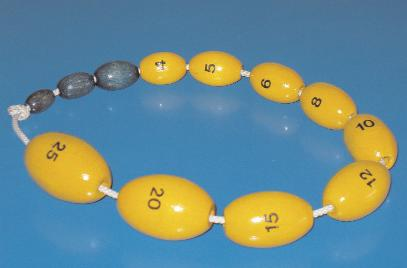
\includegraphics[scale=0.60]{grafici/orchidometro.jpg}
  \end{center}
  \caption{Orchidometro di Prader}
\end{figure}

\subsubsection*{Statura bersaglio}
Si tratta dell'altezza che ci si attende nella maggior parte dei figli sani di una coppia con una data statura. Il centro del bersaglio si ottiene nel modo seguente: per i maschi si sommano l'altezza del padre e quella della madre espressa al maschile (cioè si aggiungono 13 centimetri all'altezza materna, perchè tale è la differenza statistica fra maschi e femmine) e si divide il risultato per due; per le femmine si sommano l'altezza della madre e quella del padre espressa al maschile (vale a dire si sottraggono 13 centimetri alla statura paterna per il motivo sopra esposto) e si divide il risultato per due. 

Il centro del bersaglio $\pm$ 8 cm fornisce l'intervallo entro cui dovrebbe situarsi la maggior patre dei figli di una coppia con quella data statura.





\clearpage

\subsection{Valutazione ormonale}

\subsection{Analisi statistiche}
